\documentclass[a4paper,10pt]{article}
\usepackage[utf8]{inputenc}
\usepackage[english]{babel}
\usepackage[onehalfspacing]{setspace}
\usepackage{float}
\usepackage{biblatex}   % Using reference package
\addbibresource{mybibliography.bib}

\usepackage[nottoc]{tocbibind} %Adds "References" to the table of contents
\usepackage{graphicx}
\usepackage{hyperref}
%\graphicspath{/home/trung/Pictures/} \usepackage{float}
\hypersetup{
    colorlinks=true,
    linkcolor=blue,
    filecolor=magenta,      
    urlcolor=cyan,
}
%Document title, author and date (empty)
\title{Setting up Online Python Notebook}
\author{Trung Nguyen}
\date{}

%Beginning of the document
\begin{document}

\maketitle
\tableofcontents
\addtocontents{toc}{~\hfill\textbf{Page}\par}

\section{Introduction}

The fastest way to learn something is keep practicing. Play the whole game and learning soccer as a kids (Perkins).\\
 Skip the Introduction and go to the \hyperref[sec:Colab]{Setting up Google Colab} section.\\
When reading a scientific paper, sometimes you want to reproduce the results from the paper, or in your free time you just simply want to try something that interesting with AI application. However, you realize that running the code with your personal computer (laptop) will take a day or twos.As a result, your motivation might go down.\\
Luckily nowadays many big companies provide a basics online platform which fast enough CPU and GPU for study purposes. It means you have the possibility to use the powerful computing platform (or rent with little cost) without the need for buying a new expensive computer. 
This documents will show how to set up a few popular cloud computing platform.\\
The term GPU computing or using GPU for Deep Learning might sound familiar and also might not. Why do we need GPU for deep learning? Let first make the term a bit more clear.\\
\textbf{CPU’s (Central processing unit)} were designed as general-purpose chips that can run any application on the desktop or server. At the most basic level, the CPU can process one task at a time. Raspberry Pi is an example of an embedded device with a strong CPU.\\
\textbf{The GPU (Graphic processing unit)} makes up for the deficiency in CPU architecture by adding thousands of CUDA cores and hundreds of Tensor cores, depending on the card, that can process thousands of tasks in parallel. Nvidia Jetson is an example of a low-cost embedded device with a powerful GPU.
However, for some like Google, the GPU is still too general-purpose to run AI workloads efficiently. Thus, Google has developed its own AI hardware known as the \textbf{TPU (Tensor processing unit)}. Google describes the TPU as a “custom ASIC chip-designed from the ground up for machine learning workloads” and it currently runs many of its services like Gmail and Translates.\\
\textbf{The NPU (Neural processing unit)} is a specializes circuit that implements all the necessary control and arithmetic logic necessary to execute machine learning algorithms, typically by operating on predictive models such as artificial neural networks (ANNs) or random forests (RFs).\\
NPUs sometimes go by similar names such as a tensor processing unit (TPU), neural network processor (NNP) and intelligence processing unit (IPU) as well as vision processing unit (VPU).\\
\textbf{TPU and NPU} are more and more often use in embedded devices while GPU computing (especially NVidia GPU with Cuda cores) still dominant deep learning market for a next few years.


% ---------------------------------------------------------------------

\section{Setting up Google Colab}
\label{sec:Colab}

\href{https://colab.research.google.com/}{Google Colab} is Google's collaborative version of the Jupyter notebook. They released the tool to the general public with a noble goal of dissemination of machine learning education and research.\cite{Colab}
Users need to sign up and apply for access before using the Colab. 
To help users get familiar with the environment Google has provided a number of examples in the example tabs: 

\begin{figure}[H]
\centering
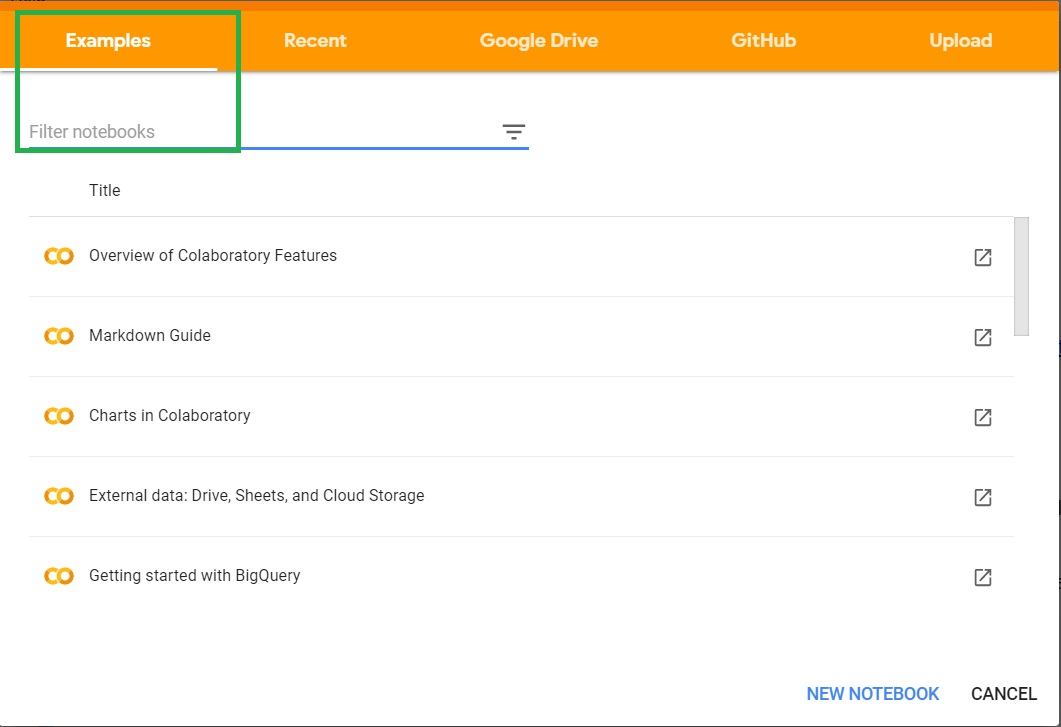
\includegraphics[width=1\columnwidth]{Pictures/Colab_interface.jpg}
\caption[Short title]{Colab interface}
\label{fig:ff1}\end{figure}

\vspace{2mm}

Select Connect on the right side of the notebook. Run the notebook by press "Shift-Enter", "Ctrl-Enter " or through the run button.    

\vspace{2mm}

\begin{figure}[H]
\centering
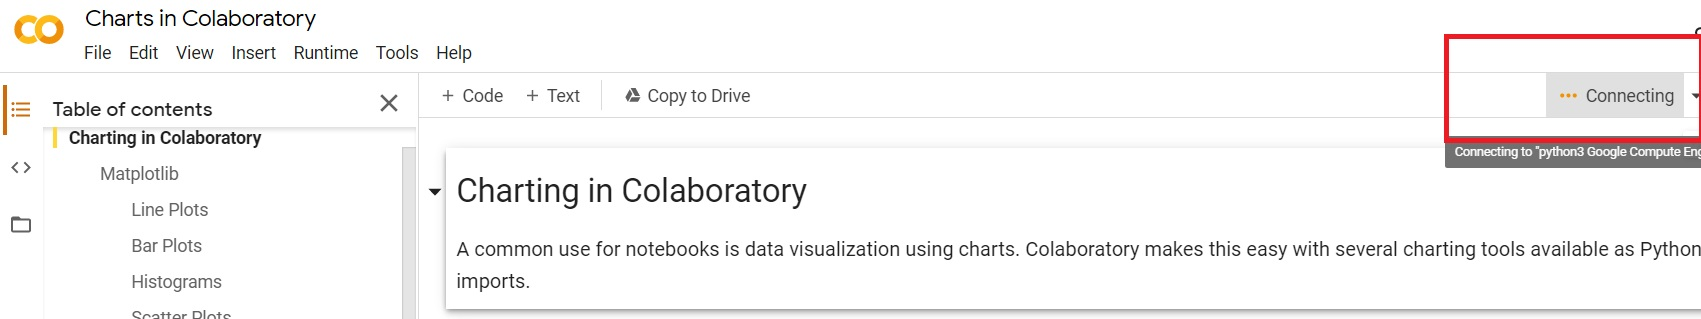
\includegraphics[width=1\columnwidth]{Pictures/Colab_Connect.jpg}
\caption[Short title]{Prepare the Notebook}
\label{fig:ff1}\end{figure}


\begin{figure}[H]
\centering
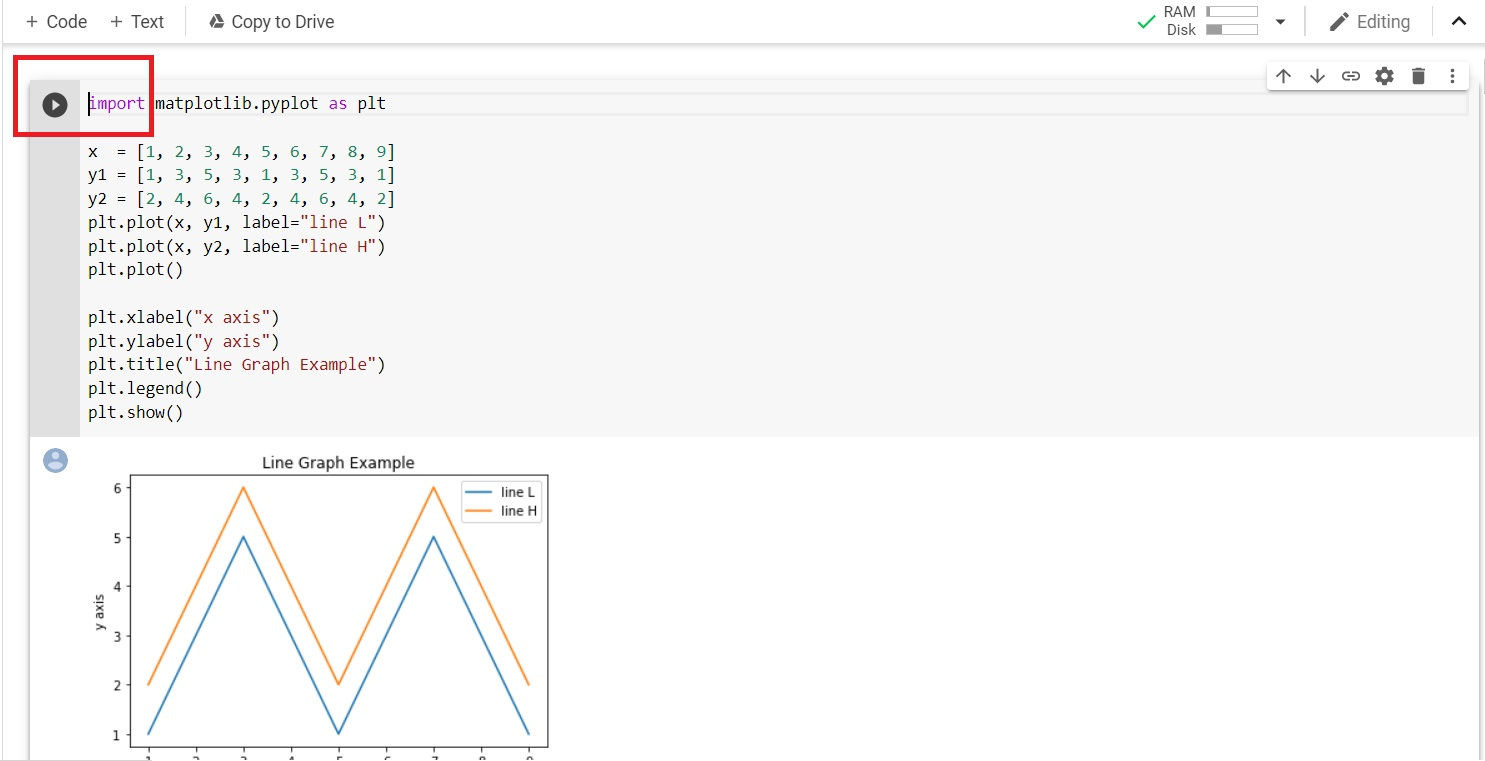
\includegraphics[width=1\columnwidth]{Pictures/Colab_Run.jpg}
\caption[Short title]{Run the Notebook}
\label{fig:ff1}\end{figure}



Setting up GPU for \href{https://colab.research.google.com/notebooks/gpu.ipynb#scrollTo=bwdaz5SIOGe9}{Google Colab}. Click the notebook setting and select GPU in the drop-down menu. Run the code to see how fast to use GPU compare with CPU. 

\begin{figure}[H]
\centering
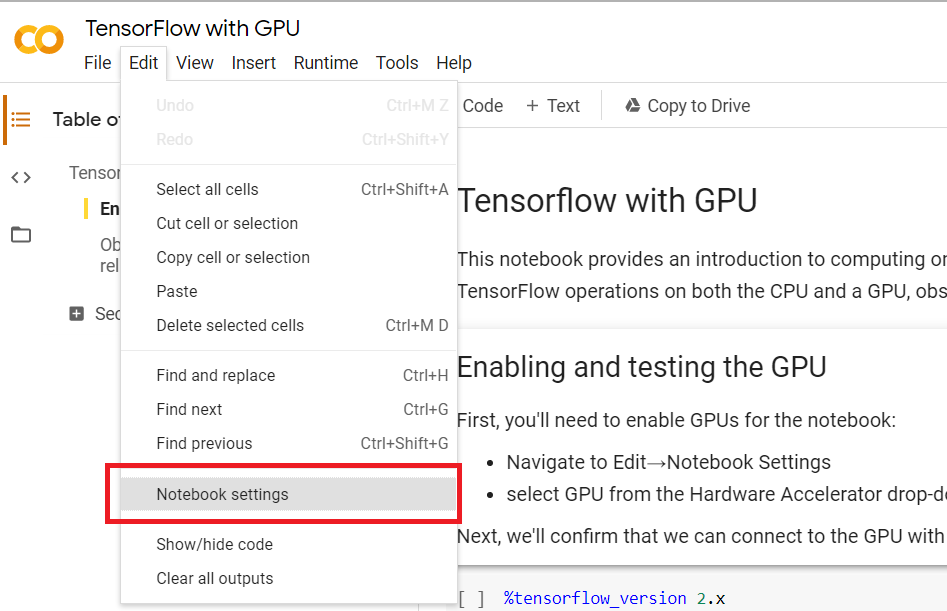
\includegraphics[width=1\columnwidth]{Pictures/Colab_set.png}
\caption[Short title]{Notebook setting}
\label{fig:ff1}\end{figure}

\begin{figure}[H]
\centering
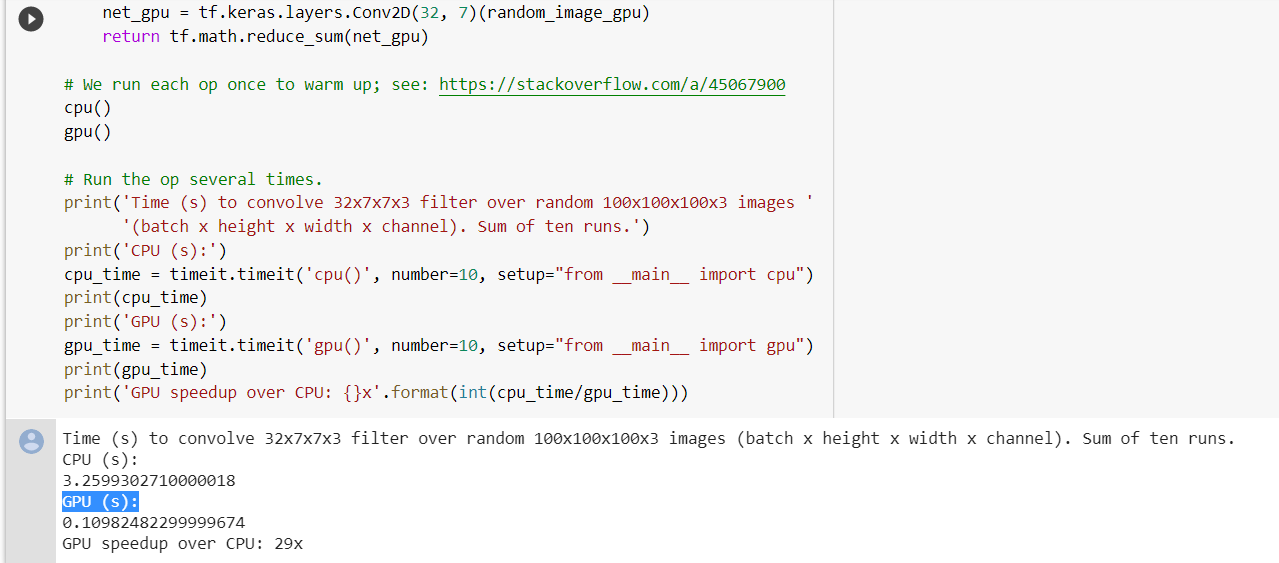
\includegraphics[width=1\columnwidth]{Pictures/Colab_gpu.png}
\caption[Short title]{GPU VS CPU}
\label{fig:ff1}\end{figure}

Run a \href{https://colab.research.google.com/drive/1cTsVAAm4pZqNgPq1A17d1pCWe1i4iIWD?usp=sharing}{Simple linear regression example using Colab} to learn more. Select save a copy in the drive, then connect and run the notebook.

\begin{figure}[H]
\centering
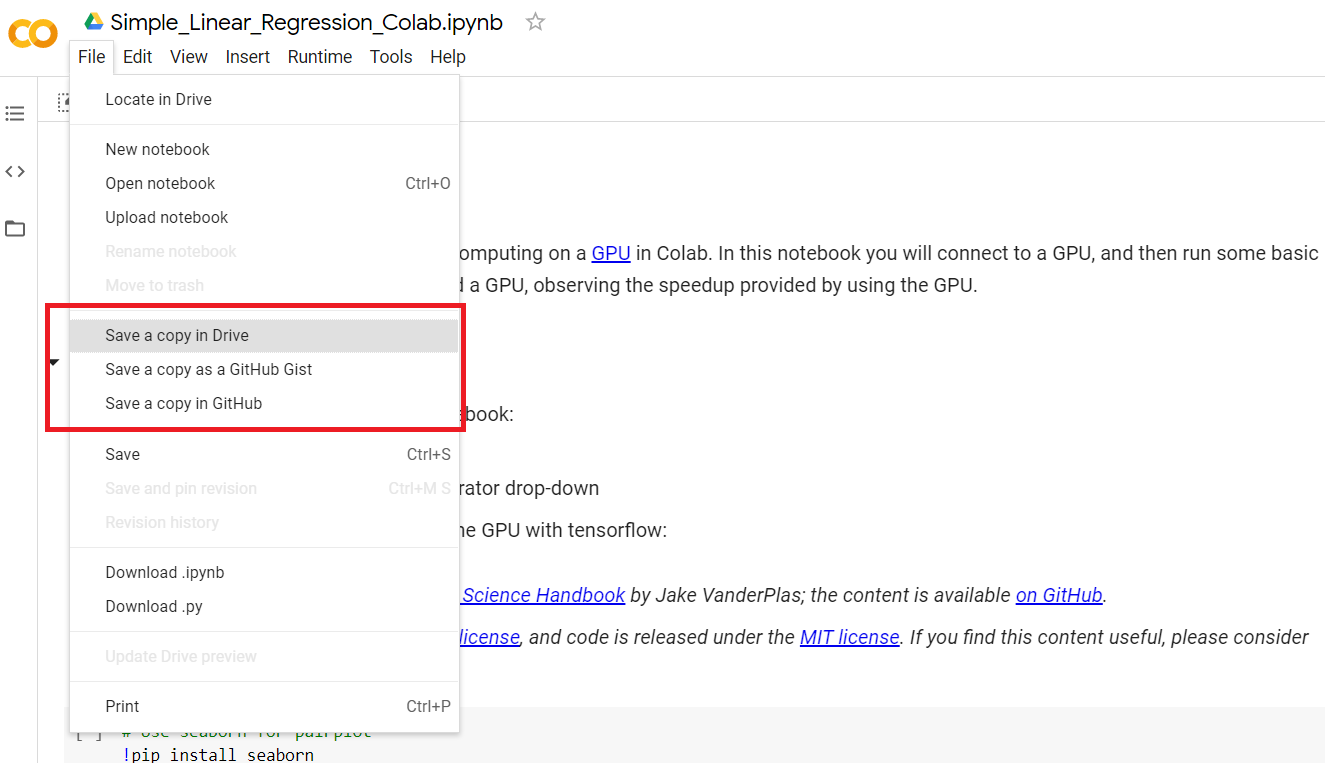
\includegraphics[width=1\columnwidth]{Pictures/Colab_savecopy.png}
\caption[Short title]{Save Copy in drive}
\label{fig:ff1}\end{figure}

\medskip

% --------------------------------------------------------------------
\newpage

\section{Run Notebook with kaggle}
Kaggle is the world's largest data science community with powerful tools and resources to help you achieve your data science goals.\cite{Kaggle}.
After creating an account with \href{https://www.kaggle.com/}{kaggle}. Select the notebook tab and create a new notebook.
\vspace{5mm}

\begin{figure}[H]
\centering
\includegraphics[width=1\columnwidth]{Pictures/kaggle_notebook.png}
\caption[Short title]{Creating notebook with kaggle}
\label{fig:ff1}\end{figure}
\vspace{5mm}

Enable GPU (only when necessary) and internet using the setting tab. kaggle only provide free 30 hours for GPU enable.  
\vspace{5mm}

\begin{figure}[H]
\centering
\includegraphics[width=1\columnwidth]{Pictures/kaggle_GPU.png}
\caption[Short title]{Enable GPU with kaggle}
\label{fig:ff1}\end{figure}

\newpage
Try \href{https://www.kaggle.com/trungnguyen0987/simple-logistic-regression-with-pytorch}{example of classification problem with kaggle}. Select copy and edit and then run the notebook example  

\begin{figure}[H]
\centering
\includegraphics[width=1\columnwidth]{Pictures/kaggle_copy.png}
\caption[Short title]{Example logistic regression notebookl}
\label{fig:ff1}\end{figure}




% ---------------------------------------------------------------------


\section{Math and Machine learning basics}
\label{sec:start}

\hspace{4ex} There are many machine learning tutorials and online courses available for free/or paid from the Internet. One of the most famous online courses for the beginner is \href{https://www.coursera.org/learn/machine-learning}{Machine Learning by Andrew.Ng from Coursera}.\\
There is also a git repository calls \href{https://github.com/trekhleb/homemade-machine-learning}{homemade machine learning} which help practicing and develop "machine learning" algorithms from scratch for better understanding of the mathematics behind each algorithm.\\  
In a git repository each algorithm has been grouped in a section which included theory, code, and practicing notebook. 

\begin{figure}[H]
\centering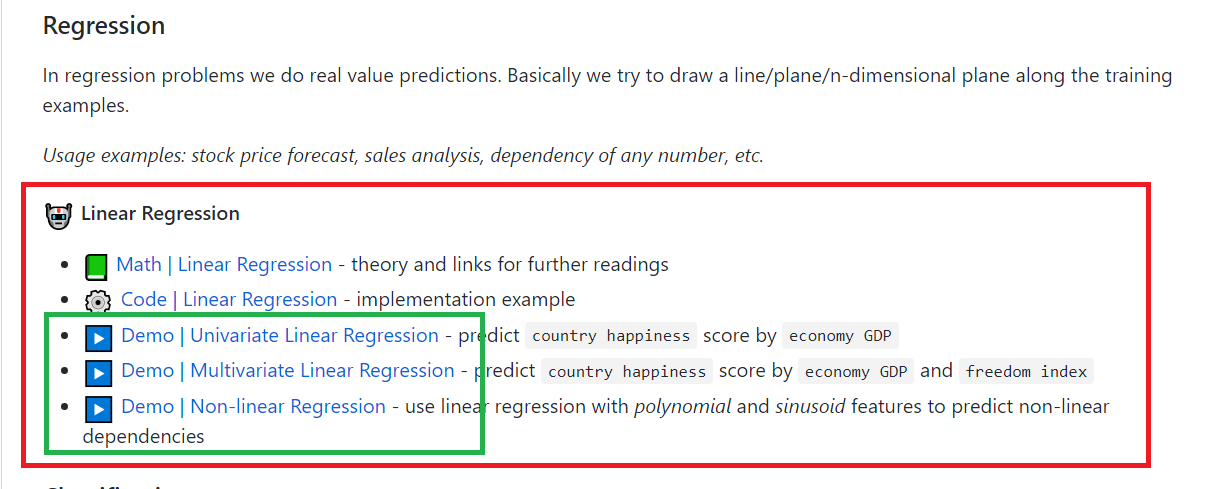
\includegraphics[width=1\columnwidth]{Pictures/HomeMade.png}
\caption[Short title]{example of group section}
\label{fig:ff7}\end{figure}

\vspace{5mm}
Click on the demo section an online Jupyter Note book will open up a running example.Click on \href{https://mybinder.org/v2/gh/trekhleb/homemade-machine-learning/master?filepath=notebooks/linear_regression/univariate_linear_regression_demo.ipynb}{" Excute on binder"} to re-run the notebook.  

\begin{figure}[H]
\centering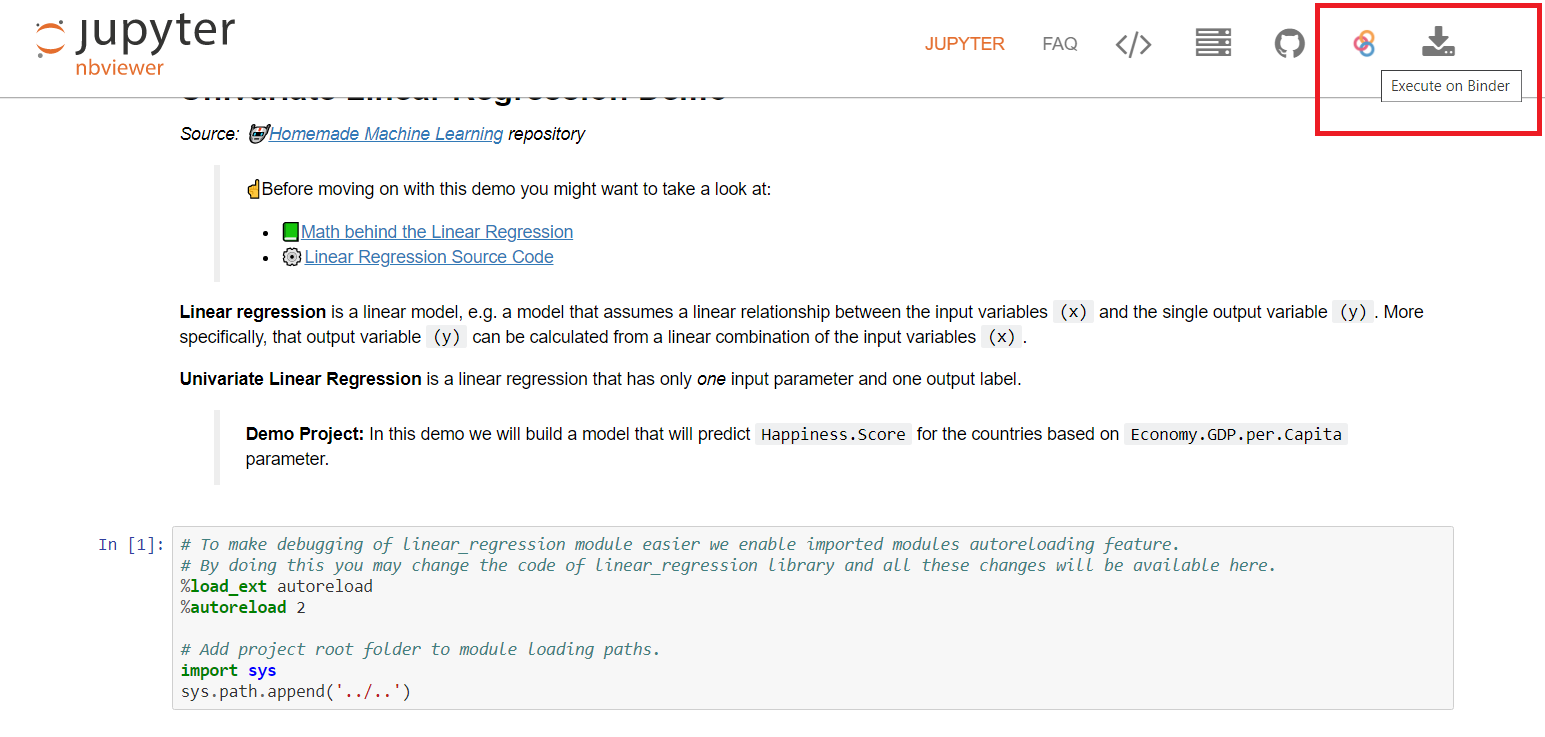
\includegraphics[width=1\columnwidth]{Pictures/Re_run.png}
\caption[Short title]{Run notebook}
\label{fig:ff7}\end{figure}

%-----------------------------------------------------------------

\section{Link to study resources}
There are many more example on Convolutional Neural Network (CNN), Recurrent Neural Networks (RNN) such as handwritten digits recognition, Shakespeare text generation,...etc on the link below.

\begin{itemize}
  \item \href{https://github.com/trekhleb/machine-learning-experiments}{Machine Learning Experiments.}
  \item \href{https://paperswithcode.com/}{Papers with code}
  \item \href{https://github.com/jakevdp/PythonDataScienceHandbook}{Python Data Science Handbook}
  \item \href{https://medium.com/deep-learning-turkey/google-colab-free-gpu-tutorial-e113627b9f5d}{Google Colab Free GPU Tutorial}.
  \item \href{https://pytorch.org/tutorials/beginner/nn_tutorial.html}{Pytorch Tutorial}

\end{itemize}



%-------------------------------------------------------------------------

\section{List of Documentation}

\begin{enumerate}
  \item Python Guideline for Beginner.
  \item Setting up Online Python Notebook
  \item update...
\end{enumerate}

\vspace{1cm}
\vspace{1cm}




%----------------------------------------------------------------

\section{Recommendation Courses}

\href{https://www.coursera.org/learn/machine-learning}{Machine learning by Andrew Ng.}\\
\href{https://www.usfca.edu/data-institute/certificates/deep-learning-part-one}{Deep Learning using FastAI  by Jeremy Howard.}


%----------------------------------------------------------------
\section{Popular Cloud Platform and their Pricing}

\href{https://gradient.paperspace.com/pricing}{Gradient.}\\
\href{https://www.onepanel.io/core/core-pricing}{Onepanel.}\\
\href{https://www.floydhub.com/pricing}{Floydhub.}\\
\href{https://cloud.google.com/pricing/list}{Google Cloud Platform.}\\
\href{https://azure.microsoft.com/en-us/pricing/details/virtual-machines/linux/}{Microsoft Azure.}\\
\href{https://aws.amazon.com/sagemaker/pricing/}{Amazon Sagemaker.}\\
\href{https://aws.amazon.com/}{Amazon AWS}
\href{https://colab.research.google.com/signup}{Google Colab Pro.}\\





%Bibliographic references
\printbibliography

\end{document}


%note 

% Upload python file to Colab
% save to drive
% import/upload data to Colab...next tutorial
% ......

% Ad Example for using Colab with Keras or Pytorch GPU train model.


% Reading \href{https://medium.com/deep-learning-turkey/google-colab-free-gpu-tutorial-e113627b9f5d}{Google Colab Free GPU Tutorial}d